\chapter{Validazione}\label{chp:validazione}
\section{Modello analitico semplificato}
Per la validazione del modello computazionale, è stata presa in considerazione una semplificazione del caso di studio originale, riportata in figura \ref{fig:validazione-modello-analitico-1} e di seguito descritta:
\begin{itemize}
\item L'insieme degli $M-1$ serventi generali viene sostituito da un singolo servente a capacità equivalente, ovvero:
\begin{equation}
C_g = (M-1)\cdot C_{g,i}
\end{equation}
\item I tempi medi di servizio per una richiesta di tipo \uo{} o \pp{} sono equivalenti e pari a:
\begin{equation}
E[S_g] = \frac{E[S_i]}{M-1} = \frac{15}{M-1}\ min
\end{equation} 
in accordo all'equazione \ref{eqn:modello-specifiche-9} ed al bullet precedente.
\item Il $\ded{}$-esimo servente, ovvero quello dedicato, non può più processare ticket di tipo \uo{} oppure \pp{} nel caso in cui non vi siano richieste \sr{} pendenti.

Ciò implica una scissione del sistema in due partizioni tra loro isolate.
\end{itemize}

\begin{figure}[ht]
\centering
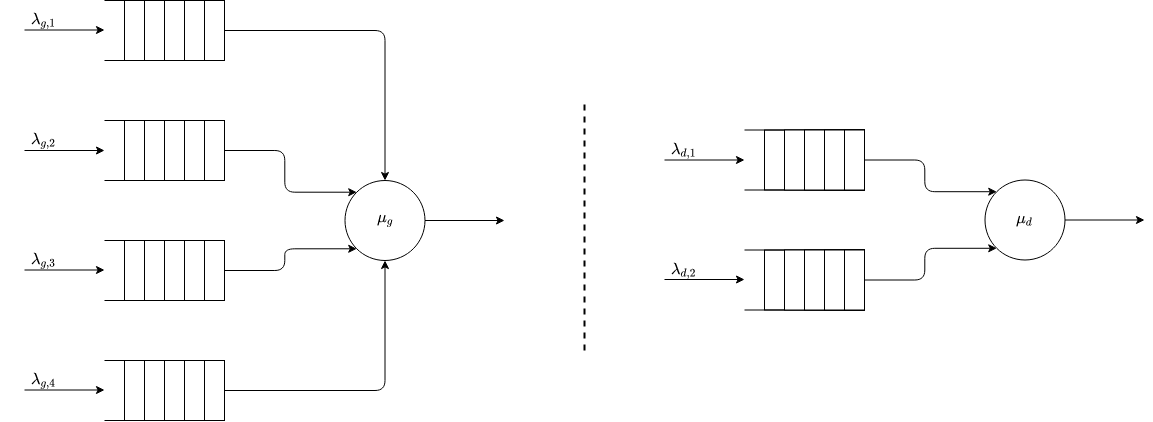
\includegraphics[width=\linewidth]{validazione-modello-analitico-1}
\caption{Rappresentazione del modello analitico semplificato}
\label{fig:validazione-modello-analitico-1}
\end{figure}

I parametri di input del sistema così semplificato sono di seguito riportati:
\begin{itemize}
\item Le probabilità di ricadere in una determinata classe sono pari a:
\begin{equation}
\begin{array}{l l}
p_{g,1} = p_{BP} \cdot p_{UO} = 0.125, & p_{g,2} = p_{BP} \cdot p_{PP} = 0.0875 \\
p_{g,3} = (1-p_{BP}) \cdot p_{UO} = 0.375, & p_{g,4} = (1-p_{BP}) \cdot p_{PP} = 0.2625 \\[1em]
p_{d,1} = p_{BP} \cdot p_{SR} = 0.0375, & p_{d,2} = (1-p_{BP}) \cdot p_{SR} = 0.1125
\end{array}
\end{equation}

I risultati ottenuti possono essere verificati con il seguente consistency check:
\begin{equation}
\sum_{i=1}^{4} p_{g,i} + \sum_{j=1}^2 p_{d,j} = 1\qquad \text{\color{forestgreen}\textbf{OK} \checkmark}
\end{equation}
\item I tassi medi d'arrivo sono pari a:
\begin{equation}
\begin{array}{l l}
\lambda_{g,1} = p_{g,1} \cdot \lambda \simeq 0.030489\ req/min, & \lambda_{g,2} = p_{g,2} \cdot \lambda \simeq 0.021342\ req/min \\
\lambda_{g,3} = p_{g,3} \cdot \lambda \simeq 0.091467\ req/min, & \lambda_{g,4} = p_{g,4} \cdot \lambda \simeq 0.064027\ req/min \\[1em]
\lambda_{d,1} = p_{d,1} \cdot \lambda \simeq 0.009147\ req/min, & \lambda_{d,2} = p_{d,2} \cdot \lambda \simeq 0.027440\ req/min \\
\end{array}
\end{equation}

I risultati ottenuti possono essere verificati con il seguente consistency check:
\begin{equation}
\sum_{i=1}^{4} \lambda_{g,i} + \sum_{j=1}^2 \lambda_{d,j} = 0.243912 = \lambda\qquad \text{\color{forestgreen}\textbf{OK} \checkmark}
\end{equation}

\item I tassi di servizio medi sono pari a:
\begin{equation}
\begin{array}{l l}
\mu_g = \frac{1}{E[S_g]} = \frac{M-1}{15}\ req/min & \mu_d = \frac{1}{E[S_d]} = 0.040196\ req/min
\end{array}
\end{equation}
dove $E[S_d] = E[S_{\ded{}, SR}]$ in accordo alla terza equazione nella \ref{eqn:modello-specifiche-12}.

\item L'occupazione media delle classi $\rho_{g,i}$ e $\rho_{d,j}$, computabile come:
\begin{equation}
\begin{array}{l l}
\rho_{g,i} = \frac{\lambda_{g,i}}{\mu_g} & \rho_{d,j} = \frac{\lambda_{d,j}}{\mu_d}
\end{array}
\end{equation}
è pari a:
\begin{equation}
\begin{array}{l l}
\rho_{g,1} = \frac{0.457335}{M-1} & \rho_{g,2} = \frac{0.320130}{M-1} \\[1em]
\rho_{g,3} = \frac{1.372005}{M-1} & \rho_{g,4} = \frac{0.960405}{M-1} \\[1.5em]
\rho_{d,1} = 0.227560 & \rho_{d,2} = 0.682655
\end{array}
\end{equation}
da cui:
\begin{equation}
\begin{array}{l l}
\rho_g = \sum_{i=1}^4 \rho_{g,i} = \frac{3.109875}{M-1} & \rho_d = \sum_{i=1}^2 \rho_{d,2} = 0.910215
\end{array}
\end{equation}
\end{itemize}

Il sistema che processa ticket di tipo \uo{} e \pp{} è modellato con una coda $M/M/1$, per cui a partire dall'analisi teorica dei modelli a classi di priorità astratta\footnote{Come nei precedenti capitoli, la priorità è inversamente proporzionale all'indice numerico della classe.}, è possibile ricavare i seguenti indici:
\begin{itemize}
\item Il \textbf{tempo d'attesa} dell'$i$-esima classe, con $i\in\lbrace 1, 2, 3, 4\rbrace$ è pari a:
\begin{equation}
E[T_{Q_{g,i}}] = \frac{\rho_g E[S_g]}{\left(1- \sum_{k=1}^{i} \rho_{g,k}\right)\left(1- \sum_{k=1}^{i-1} \rho_{g,k}\right)}
\end{equation}
da cui:
\begin{equation}
\begin{cases}
E[T_{Q_{g,1}}] = \frac{46.6481}{M - 1.45734}\ min \\[1em]
E[T_{Q_{g,2}}] = \frac{46.6481\cdot (M-1)}{M^2 - 3.2348\cdot M + 2.59036}\ min \\[1em]
E[T_{Q_{g,3}}] = \frac{46.6481\cdot (M-1)}{M^2 - 4.92694\cdot M + 5.59807}\ min \\[1em]
E[T_{Q_{g,4}}] = \frac{46.6481\cdot (M-1)}{M^2 - 7.25935\cdot M + 12.9439}\ min
\end{cases}
\end{equation}
\end{itemize}